\chapter{序論} % 章のタイトル

% \includegraphics[width=??cm]{hoge.eps} % 図(EPS形式)を読み込む場合

\section{背景} % sectionのタイトル

% 以下に背景,関連する環境状況,技術に関する概要を記述.

近年,インターネット技術やセンサー技術の進化を背景に,パソコンやスマートフォンなどのインターネット端末に加え,家電や自動車などの様々なものに通信機能を搭載したIoTデバイスが普及し始めている.総務省によると政界中のIoTデバイスの数は図1のように2017年時点でIoTデバイスが約275億台存在し,2020年にはIoTデバイスが403億台に及ぶと予想されている\cite{IoT}.
 \begin{figure}[h]
 \centering
    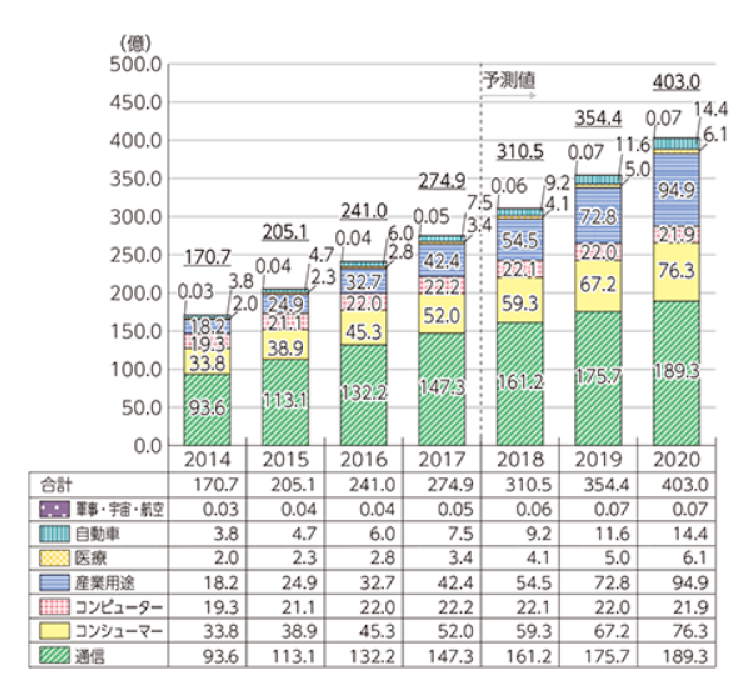
\includegraphics{figures/IoT_device.eps}
 \label{fi:model}
 \begin{center}図1 世界のIoTデバイス数の推移及び予測\end{center}
 \end{figure}
%参考文献をしっかり入れ直す
IoTデバイスの普及に伴い,IoTデバイスを対象としたマルウェアが急増している.
IoTデバイスの重要な問題の1つとしてセキュリティ問題が挙げられる.IoTデバイスのユーザ名やパスワードを初期設定の状態で使用する場合が多いことやデバイスの資源が限られていることから,セキュリティが十分に考慮されていない事がある.そのため,IoTデバイスを対象としたマルウェアが脅威となっている.その中でもネットワークサービスを停止させる深刻な問題を引き起こしているマルウェアにはDDoS(Distributed Denial of Service)攻撃を行っているものが多く存在し,その対策が重要視されている.DDoS攻撃は,攻撃者が複数の他人のコンピュータを利用し,公開されているサービスに大量のデータを送りつける事によって処理負荷を与えサービスを機能停止に追い込む攻撃である.代表的なDDoS攻撃を行うマルウェアとしてMiraiが挙げられる.Mirai\cite{Mirai}は,無作為なIPアドレスから感染できるデバイスを探し出し,ログイン可能なデバイス上に,悪意のあるソフトウェアをダウンロードし実行させることでそのデバイスを制御下に置く.攻撃者によって制御された端末は他に侵入可能な端末を探し出し,次々と感染させることでボットネットと呼ばれる悪意あるプログラムを使用して乗っ取った多数のコンピュータで構成されるネットワークを構築する.その後,C\&C(Command and Control)サーバから送られた指示に対してDDoS攻撃を行うマルウェアである.2016年10月に発生した,DNSサーバープロバイダであるDyn社へのDDoS攻撃ではIoTデバイスによるボットネットが利用され史上最大規模である620Gbpsの攻撃が観測された\cite{Dyn}.その後,Miraiのソースコードが公開され,Owari,Satori,OkiruといったMiraiの亜種の開発が盛んに行われるようになった.MiraiやMirai亜種のマルウェアによって,多くのIoTデバイスがDDoS攻撃に不正利用されるようになったことから,国立研究開発法人情報通信研究機構がパスワード設定などに不備のあるIoT機器の実態把握を目的として日本国内のIPv4アドレスを対象にSSH,Telnet,HTTPであるTCPの22番,23番,80番ポートを対象にポートスキャンを行ったcite{国立}.
%ここ少しおかしいから治す
IoTデバイスの不正利用によるDDoS攻撃が注目されている.

\section{IoTデバイスで検知を行う必要性}

IDS(Instrusion Detection System)と呼ばれる不正な通信やホストへの侵入,ファイルの改ざん等の不正な侵入の兆候を検出するシステムの設置場所として2種類が考えられる.ネットワーク上に設置するネットワーク型と端末上に設置するホスト型の2種類が考えられる.ネットワーク型のIDSでは,ネットワークに流れるデータを取得して解析し,異常がないか確認する.不正が疑わ得れるデータを検知したときには管理者に知らせる.しかし,ネットワーク上でネットワークトラフィックからDDoS攻撃を判別するのは難しく誤検知する可能性が考えられる.しかし,マルウェアに基づいて作成されたデータを用いたパターンマッチングによる検知手法では,誤検知率が低く既存のマルウェアを確実に検知できる利点が有る.公開されているソースコードを基に作成されたマルウェアは,オリジナルのマルウェアと共通するシグネチャが存在すると考えられるためパターンマッチングによる検知で亜種のマルウェアにも対応できると想定される.脅威となっているマルウェアは,十分に管理が行われていないIoTデバイスで散見される,放置された初期パスワードのままのアカウントや,保守されていないシステムの脆弱性をついた攻撃を行うため,侵入されてしまうことは前提とすべきである.そのため,デバイスの性能が限られているIoTデバイス上でもマルウェアの検知を行う必要がある.

\section{マルウェアMiraiの概要}

Miraiは,ネットワーク上で公開されているLinuxで動作するデバイスを不正利用し,DDoS攻撃を行うマルウェアである.ネットワークカメラやルータといったIoTデバイスをターゲットにしている.Miraiは,C\&Cサーバー,MySQL,Loader,botの4つから構成される.Miraiの概要を図2に示す.

\begin{figure}[h]
   \centering
      
\includegraphics[width=150mm]{figures/test.eps}
   \label{fig:model}
   \begin{center}図2 Miraiの概要図\end{center}
\end{figure}

C\&Cサーバーは,ボットやユーザーからの接続されるのを待機しており,主な機能としてボット管理機能,ユーザー管理機能,攻撃指示機能がある.MySQLにはユーザーのリストと攻撃履歴が記録されるようになっている.botは,C\&Cサーバーからのコマンドを待機し,感染先でボットネットに加えられる新しいデバイスを探索するスキャン活動を行う.スキャン活動を行いログインできる端末を見つけた場合には,IPアドレス,ポート,ログイン情報をスキャンサーバーへと送る.感染経路について,Miraiは、Telnetログインが可能な場合に感染する.Loaderは,スキャン活動からレポートサーバーに送られた攻撃対象の情報をもとにTelnetログインを試みる.Telnetログインに成功した際には,攻撃者が用意したhttpサーバーまたはtftpサーバーから,Miraiのバイナリファイルを対象のIoTデバイスにダウンロードしbotを実行させる.botの動作後には,C\&Cサーバーとの通信を始め,C\&Cサーバーから送られてくる攻撃命令を受け取り,IoTデバイスが特定のサーバーに攻撃を始める
.攻撃種類としては,~~~~~

\section{研究目的}
本研究では,DDoS攻撃を行うマルウェアMiraiとその亜種の未知のマルウェア検知である.

\section{論文の構成}
本論文は,